\chapter{网络}

\section{因特网}

\subsection{因特网(Internet)}

因特网是一个世界范围的计算机网络,它互联了遍及全世界数十亿的计算设备,所有这些设备都称为主机(host)或端系统(end system)。端系统通过通信链路(communication link)和分组交换机(packet switch)连接到一起,不同的链路能够以不同的速率传输数据,链路的传输速率(transmission rate)使用比特/秒(bps, bit/s)来度量。端系统通过因特网服务提供商(ISP, Internet Service Provider)接入因特网。\\

当一台端系统向另一台端系统发送数据时,发送端将数据分组,发送到目的端系统,在那里进行组装。一个分组所经历的一系列通信链路和分组交换机称为路径(route / path)。分组交换类似于现实中的货物运输,在出发地将货物分开并装上多辆卡车,每辆卡车独立通过公路运输,最后在目的地卸货并重新组装。

\begin{figure}[H]
    \centering
    \includegraphics[scale=0.8]{img/C1/1-1/1.png}
    \caption{计算机网络}
\end{figure}

\vspace{0.5cm}

\subsection{分布式应用程序(Distributed Application)}

分布式应用程序涉及多个相互交换数据的端系统,例如即时通信、实时道路信息、视频会议、多人游戏等。分布式应用程序的核心问题在于一个端系统上的应用程序如何能够向运行在另一个端系统上的应用程序发送数据。\\

套接字接口(socket interface)规定了运行在一个端系统上的程序向运行在另一个端系统上的特定程序交付数据的方式。例如Alice要给Bob寄一封信,当然Alice不能只是写完这封信就把它丢出窗外。Alice需要把信放入信封,在信封上根据指定格式写上收信人的全名、地址和邮政编码,信封上贴上邮票,再将信封投入信箱中。Alice想要寄信就必须要遵守邮政服务制定的这一套规则。因此,发送数据的程序也必须遵守socket接口,才能向接收数据的程序发送数据。\\

\subsection{协议(Protocol)}

在两个人或两台设备之间进行通信时需要遵守一些协议,协议就是用于管理通信的一组规则。传输控制协议TCP(Transmission Control Protocol)和网际协议IP(Internet Protocol)是因特网中两个最为重要的协议,因特网的主要协议统称为TCP/IP。\\

因特网标准(Internet standard)是经过充分测试的规约,只要是与因特网打交道,就会用到它们,并要服从于它们。因特网标准由IETF(Internet Engineering Task Force)研发,IETF的标准文档称为RFC (Request For Comment),目的是解决因特网先驱者们面临的网络和协议问题。它们定义了TCP、IP、HTTP、SMTP等协议,目前已经有将近7000个RFC。\\

人类无时无刻都在执行协议,人类用约定好的交互方式互相交流。但是如果两人的交谈都不在同一频道上,那就不能好好沟通了。\\

\begin{figure}[H]
    \centering
    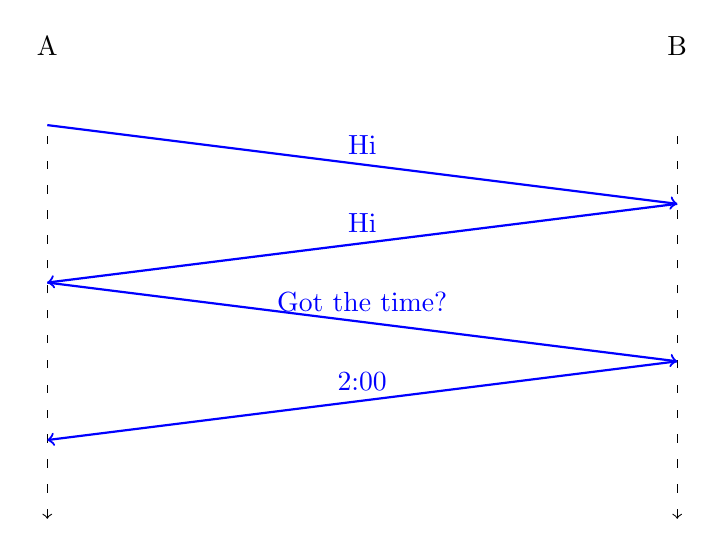
\begin{tikzpicture}
        \node at (0,6) {A};
        \node at (8,6) {B};

        \draw[loosely dashed, <-] (0,0) -- (0,5);
        \draw[loosely dashed, <-] (8,0) -- (8,5);

        \draw[blue, ->, thick] (0,5) -- (4,4.5) node[above]{Hi} -- (8,4);
        \draw[blue, ->, thick] (8,4) -- (4,3.5) node[above]{Hi} -- (0,3);
        \draw[blue, ->, thick] (0,3) -- (4,2.5) node[above]{Got the time?} -- (8,2);
        \draw[blue, ->, thick] (8,2) -- (4,1.5) node[above]{2:00} -- (0,1);
    \end{tikzpicture}
    \caption{人类协议}
\end{figure}

在因特网中,涉及两个或多个远程通信实体的所有活动都受协议的制约。例如在浏览器中输入URL(Uniform Resource Locator)向一个Web服务器发出请求,首先你的计算机将向该Web服务器发送一条连接请求报文,并等待回答。Web服务器接收到连接请求报文,并返回一条连接响应报文。在得知请求正常后,计算机会发送一条要获取的网页名字的报文,最后Web服务器向计算机返回该网页。\\

\begin{figure}[H]
    \centering
    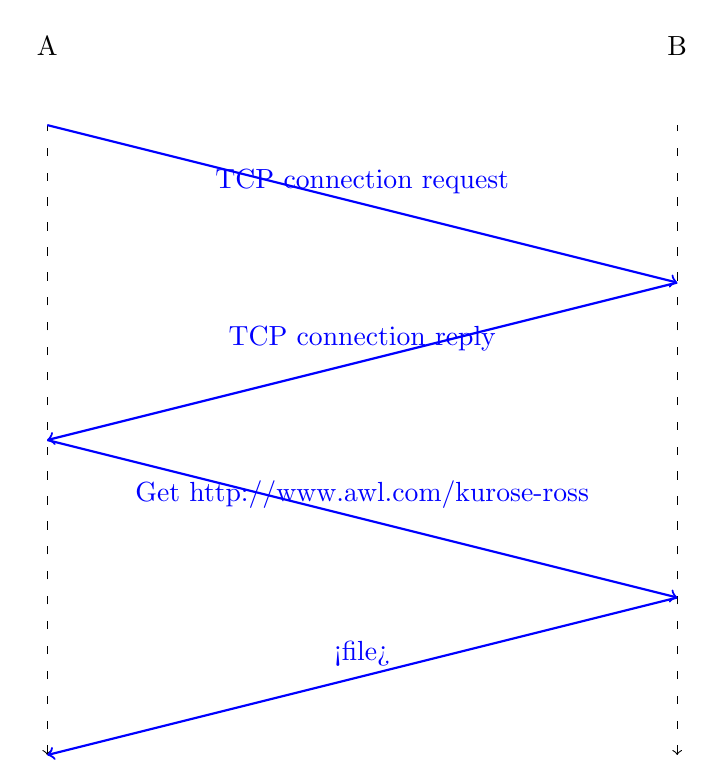
\begin{tikzpicture}
        \node at (0,9) {A};
        \node at (8,9) {B};

        \draw[loosely dashed, <-] (0,0) -- (0,8);
        \draw[loosely dashed, <-] (8,0) -- (8,8);

        \draw[blue, ->, thick] (0,8) -- (4,7) node[above]{TCP connection request} -- (8,6);
        \draw[blue, ->, thick] (8,6) -- (4,5) node[above]{TCP connection reply} -- (0,4);
        \draw[blue, ->, thick] (0,4) -- (4,3) node[above]{Get http://www.awl.com/kurose-ross} -- (8,2);
        \draw[blue, ->, thick] (8,2) -- (4,1) node[above]{<file>} -- (0,0);
    \end{tikzpicture}
    \caption{网络协议}
\end{figure}

\newpage